\chapter{Overview of system}
\label{ap:systemOverview}
\graphicspath{{Chapter1/Chapter1Figures/},{Chapter4/Chapter4Figures/}}

In this chapter a graphical and mathematical derivation of the entire system is given.

\section{System as a whole}

\begin{figure}
  \centering
  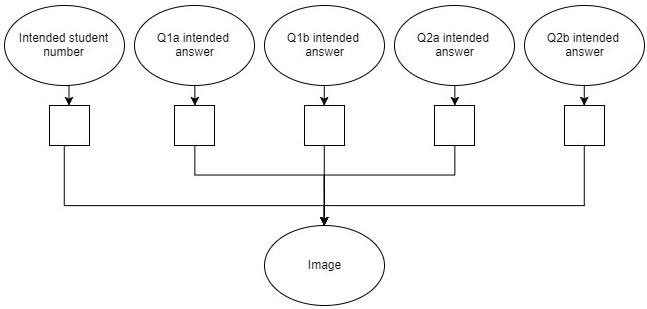
\includegraphics[width=11cm]{systemOverview}\\
  \caption{System overview.}
  \label{fig:systemOverview}
\end{figure}

As described in Chapter \ref{ch:Introduction}, the system can fundamentally be represented with 6 information nodes. These nodes are shown in Figure \ref{fig:systemOverview}. The student has certain information he/she wants to portray on the paper. This includes the 4 answers and student number the student wants to write down. Thus those 5 nodes gives rise to the image, representing the last node. Thus fundamentally the system is tasked with working out these 5 conditional probabilities: $P(StudentNumber/Image)$, $P(Answer1/Image)$, $P(Answer2/Image)$, $P(Answer3/Image)$ and $P(Answer4/Image)$. The random variables StudentNumber and Answer(1 to 3) thus represent all the possible values that the student number and answers possibly can be. The Image is a random variable representing the total number of possible states the image can represent. This value is in the order of 1240*1754*256 possible states. To practically represent this further assumptions are made in the following sections. 
 
The aim of the software is to maximize the likelihood of those probability distributions indicating the correct answers.
The reason the problem is represented in a probabilistic way is due to the fact that different images are going to be generated every time a test is written. This is true even when the same information is going to be portrayed. Everytime a student writes a test he/she is going to write in different ways. A probabilistic graphical model (PGM) is thus used to describe this system and its inner operations. For a more detailed explanation on PGM's, refer to Section \ref{sec:PGM}.  The blocks in Figure \ref{fig:systemOverview} represent additional processing that is described in the following sections.

To calculate those 5 probabilities, some more detailed derivations are necessary. These derivations are described in the next section.

\section{Deriving the intended student entry}

\subsection{Student answer}



To determine a answer for one of the students questions, $P(Answer2/Image)$, so further derivations and assumptions are necessary. There are 8 possible columns to use for an answer. The first column defecates the sign of an answer. Thus two signs are possible. For each of the remaining 7 columns a number from 0 - 9 can be represented. Thus there are ten possible values for each column. This gives a possible number of values to search through to be $2*10^7 = 20 000 000$. Each of these states needs to be calculated and thus is computationally intractable. Thus a assumption is needed to reduce the number of possible states. A fair assumption to made, all $20 000 000$ possible numbers are equally likely to be written down. Thus each column digit becomes independent of the another columns. Thus if a value in one column is known, it does not influence the probabilities of the other columns being a certain value. Thus the number of states no becomes $2+10*7=72$, which is significantly less. and An illustration of this graph can be seen in Figure \ref{fig:ans}. In Equation \ref{eqn:ansIndep} this independence property can now be seen. To find the most probable answer only $P(sign/Image)$ and $P(digit(1-7)/Image)$ still needs to be calculated. Using the image processing techniques described in Section \ref{ch:ImageProcessing} the $P(sign/Image)$ can simply be determined heuristically by determining the probability of the bubble being coloured in, underneath the sign. Thus the only values yet to calculate is $P(digit/Image)$. This is described in Section \ref{sec:digit}.

\begin{align}
% \nonumber to remove numbering (before each equation)
  P(Answer/Image) =  P(sign/Image)*P(digit1/Image)*...*P(digit7/Image)
\label{eqn:ansIndep}
\end{align}

\begin{figure}
  \centering
  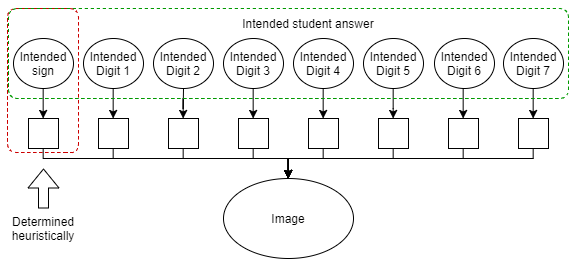
\includegraphics[width=10cm]{ans}\\
  \caption{Graphical setup of determining student answer.}
  \label{fig:ans}
\end{figure}

\subsection{Student number}

The previous assumption does not hold in the case of student numbers. Knowing the digit value of one column changes the probability of each other column taking a certain value. The reason for this is, because there is only a limit number of student numbers to consider. Thus if the first digit is a 2, only student numbers starting with 2 must still be considered. To account for this fact an additional node is added above the individual digit probabilities. This node represents the probability of each student number being present in the image. This node will have $+- 900$ states, depending on the number of student numbers. The student number graph can be seen in Figure \ref{fig:stdNum}. Next a derivation for $P(studentNumber/Image)$ is needed. 

In the below equations, 'Digits' represents the 8 digit random variables. The first step is to apply Bayes rule as seen in Equation \ref{eqn:bayesStd}.

\begin{align}
  P(StudentNumber,Digits/Image) =  \frac{P(Image/StudentNumber,Digits)*P(StudentNumber,Digits)}{P(Image)}
\label{eqn:bayesStd}
\end{align}

When all the digits are known, the image becomes independent of the student number. This can be seen in Equation \ref{eqn:bayesStd}. Also the chain rule stats that Equation \ref{eqn:chain} must be true.

\begin{align}
  P(Image/StudentNumber,Digits) = P(Image/Digits)
\label{eqn:digitInd}
\end{align}

\begin{align}
  P(StudentNumber,Digit) = P(Digit/StudentNumber)*P(StudentNumber)
\label{eqn:chain}
\end{align}

Next the Digit random variable is summed out to produce $P(studentNumber/Image)$, as seen in Equation \ref{eqn:sumRule}.

\begin{align}
  P(StudentNumber/Image) = \sum_{D}^{All} \frac{P(Image/Digits)*P(Digit/StudentNumber)
  *P(StudentNumber)}{P(Image)}
\label{eqn:sumRule}
\end{align}

Applying Bayes rule again the following equality can be presented, as seen in Equation \ref{eqn:bayesStd2}.

\begin{align}
  P(StudentNumber/Image) = P(Image/Digits) = \frac{P(Digits/Image)*P(Image)}{P(Digits)}
\label{eqn:bayesStd2}
\end{align}

Thus the result can be seen in Equation \ref{eqn:final}. $P(StudentNumber)$ can be taken out of the sum, due to it being independant of $Digits$.

\begin{align}
  P(StudentNumber/Image) = P(StudentNumber)*\sum_{D}^{All} \frac{P(Digits/Image)
  *P(Digits/StudentNumber)}{P(Digits)}
\label{eqn:final}
\end{align}

$P(StudentNumber)$ can be initialized as a equal distribution, because every student number is equal as likely to be in a given test. $P(Digits/StudentNumber)$ is a value that is trained from data. This value symbolizes the probability that the user intended to write down a given digit given that student's student number. This number is thus strongly correlated with the student number. If the first digit of the student number is 1, Digit1 will have a high probability of being 1. The only values that still needs to be calculated are thus $P(Digits/Image) = P(Digit1/Image)*...*$. This derivation is covered in the next section.

\begin{figure}
  \centering
  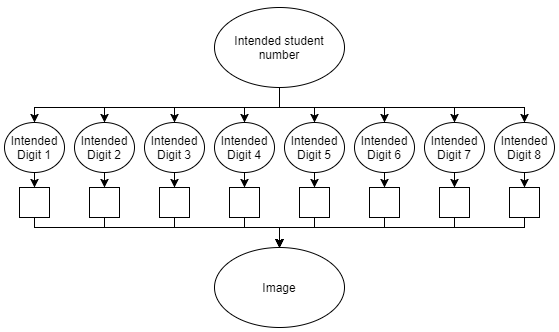
\includegraphics[width=10cm]{stdNum}\\
  \caption{Graphical setup of determining student number.}
  \label{fig:stdNum}
\end{figure}

\section{Deriving the estimated digit}
\label{sec:digit}



\begin{figure}
  \centering
  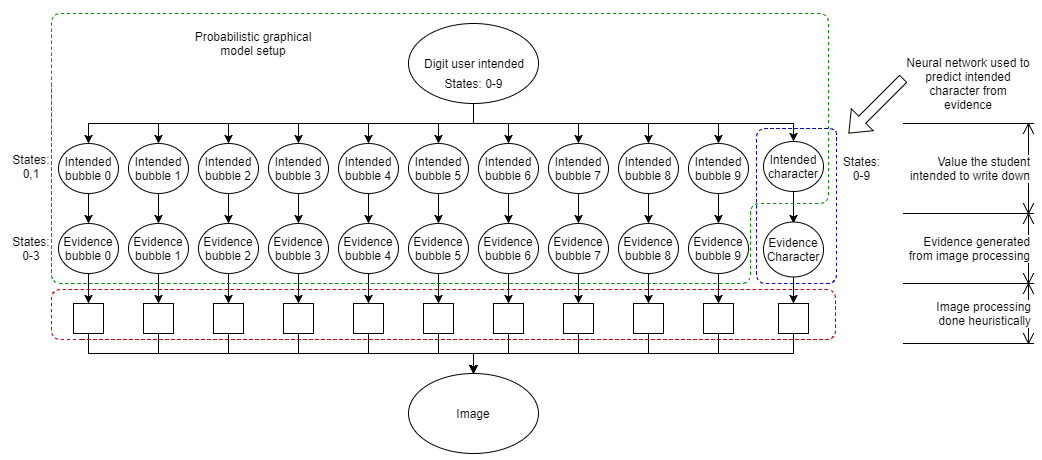
\includegraphics[width=16cm]{pgmDigit}\\
  \caption{Graphical setup of determining intended digit.}
  \label{fig:pgmDigit}
\end{figure}
